\section{Task models}

A task is an independent thread of execution that can compete with
other concurrent tasks for processor execution time.
A task is defined by a set of parameters and supporting data structures.

\begin{itemize}
	\item A name
	\item A unique ID
	\item A priority
	\item A task control block
	\item A stack
	\item A task routine
\end{itemize}



Criteria for task creation:

\begin{itemize}
	\item{Parallelism: Simultaneous and independent functionality}
	\item{Timing: Different timing constraints}
	\item{Priority: Divide tasks with different priority}
	\item{Structure: Each task handles one well defined problem}
	\item{Coupling: Divide problem into loosely coupled tasks.}
	\item{Periodicity: A task that must execute with a fixed period is a task by itself.}
\end{itemize}

\begin{center}
	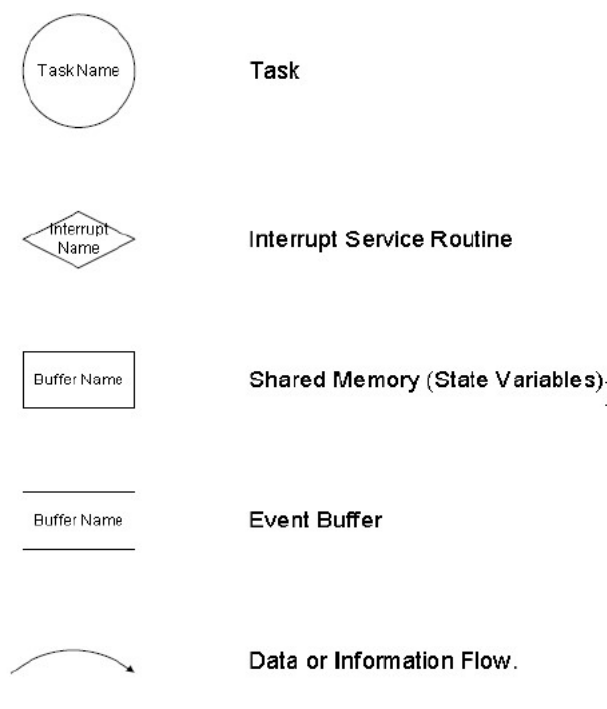
\includegraphics[width=0.4\textwidth]{images/taskDiagramComponents.png}
\end{center}

A shared memory element keeps its value after it has been read.
An event from the event buffer gets destroyed after reading and processing.

The differentiation between state machines and task models is that
task models describe multiple tasks and the flow of information between them
which can run in parallel. State machines describe the single thread of
execution based on states and transitions between them.

\textbf{Shared memory:} Keeps its value after it has been read.

\textbf{Event buffer:} Gets destroyed after reading and processing.


\begin{center}
	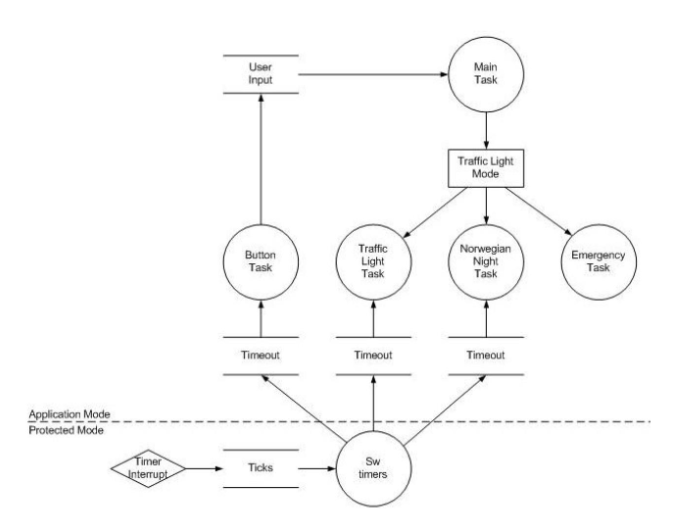
\includegraphics[width=\textwidth]{images/taskmodel2.png}
\end{center}
